\section{Quadrature}

The central building block for evaluating inner products is the calculation of
integrals between wavepackets.
This is done numerically with a quadrature rule, of which there are many
different kinds.


\subsection{Gauss-Hermite Quadrature}

The basic integration algorithm used in this project is the one-dimensional
Gauss-Hermite quadrature.
Like related rules, this method works by evaluating the integrand function at a
defined set of nodes $\gamma_i$, the values of which are summed up with specific
weights $\omega_i$:

\begin{equation}
  \label{eq:gaussquad}
  \int_{-\infty}^{\infty} g(x) \, dx \approx \sum_{i=1}^{n} f(\gamma_i) \omega_i
\end{equation}

In its basic form, the Gauss-Hermite rule works on special integrals of the
following form:

\begin{equation}
  \int_{-\infty}^{\infty} e^{-x^2} f(x) \, dx
\end{equation}

However, as we require the quadrature to work on general functions,
transformations are done to the usual weights and nodes which is described in
\cite{B_master_thesis}.
The result is a rule in the form of \eqref{eq:gaussquad}.
Figure~\ref{fig:ghexample} shows an example of the node distribution of a
Gauss-Hermite rule.

\begin{figure}
  \center
  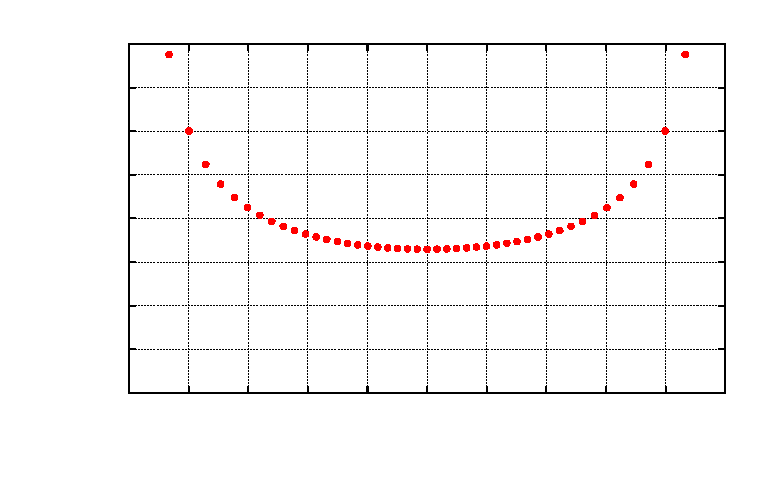
\includegraphics[width=\linewidth]{figures/gh-rule.eps}
  \caption{45-point Gauss-Hermite nodes and weights}
  \label{fig:ghexample}
\end{figure}

In the implementation of this rule, an auxiliary Python script was made to
automatically generate C++-code with hardcoded tables of nodes and weights for
different orders.


\subsection{Tensor-Product Quadrature}

The wavepackets that are processed by WaveBlocks are generally multi-dimensional.
To handle this, tensor products of $D$ one-dimensional quadrature rules can be
built up.

Denoting the $i$-th node-weight-pair of the $d$-th scalar quadrature rule
$(\gamma_i^d,\ \omega_i^d)$, the resulting pair at the multi-index $j = (j_1,
\ldots, j_d)$ for the resulting tensor quadrature rule is:

\begin{equation}
  (\gamma_j,\ \omega_j) = \left(
    \begin{pmatrix} \gamma_{j_1}^1 \\ \vdots \\ \gamma_{j_d}^d \end{pmatrix},
    \ \prod_{d=1}^D \omega_{j_d}^d
  \right)
\end{equation}
